\def\QRCODE{TB_IPR_TUT.IMG.harris_detector_pythonqrcode.png}
\def\QRPAGE{http://www.iptutorials.science/tree/master/TB_IPR/TUT.IMG.harris_detector/python}
\pcorrectionsection{Python correction}


\subsection{Cornerness measure}

\begin{figure}[H]
 \centering\caption{Cornerness measure for the checkerboard image. The next step is to locate the corners by thresholding the measure, extracting the local maxima, eliminating points near the edges...}%
 \subfloat[Checkerboard.]{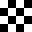
\includegraphics[width=.3\linewidth]{checkerboard.python.png}}\hfill
 \subfloat[Cornerness measure.]{
\includegraphics[width=.3\linewidth]{cornerness_checker.python.png}}\hfill
 \subfloat[Harris corner points.]{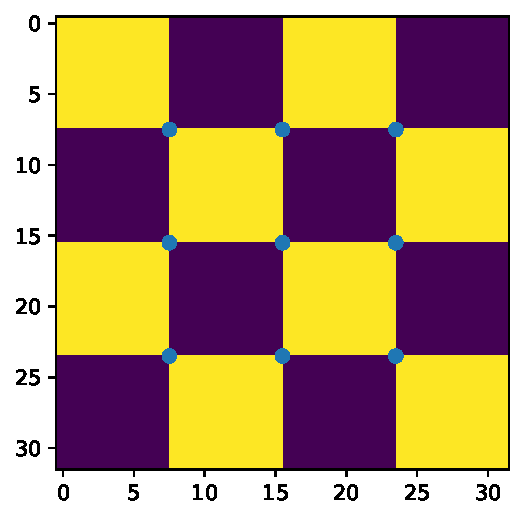
\includegraphics[width=.3\linewidth]{harris_checker.python.pdf}\label{fig:harris:python:cornerness:harris}}%
 \label{fig:harris:python:cornerness}%
\end{figure}

The first step is to compute the gradient in both x and y directions.
\begin{python}
Ix = scipy.ndimage.sobel(I, axis=0);
Iy = scipy.ndimage.sobel(I, axis=1);
\end{python}

Then, the coefficients of the matrix are computed.
\begin{python}
M1 = np.multiply(Ix, Ix);
M2 = np.multiply(Iy, Ix);
M4 = np.multiply(Iy, Iy);
\end{python}

In case of using a scale parameter, these coefficients should be filtered (for example via a gaussian filter).
\begin{python}
M1 = scipy.ndimage.gaussian_filter(M1, sigma);
M2 = scipy.ndimage.gaussian_filter(M2, sigma);
M4 = scipy.ndimage.gaussian_filter(M4, sigma);
\end{python}

Finally, the cornerness measure is evaluated.
\begin{python}
C = (np.multiply(M1, M4) - np.multiply(M2, M2)) - K * np.multiply(M1+M4, M1+M4);
\end{python}

The cornerness measure is displayed in Fig.\ref{fig:harris:python:cornerness}.

\subsection{Corners detection}

In order to keep only the strongest corner points, a threshold value $t$ is applied on $C$. This value is really depending on the considered image, thus such a global threshold is not generally a good idea. One would probably prefer a h-maximum or equivalent operator. For the purpose of this tutorial, we will keep this strategy.

\begin{python}
C[C<t] = 0;
\end{python}

The local maxima are then extracted.
\begin{python}
corners = peak_local_max(C, indices=False, min_distance=2);
\end{python}


The result is a binary image, where some clusters of points are the corner points. To keep only one point per cluster, the centroid of each is detected. The final result is presented in Fig.\ref{fig:harris:python:cornerness:harris}.
\begin{python}
L = measure.label(corners);
props = measure.regionprops(L);
centers=[];
for prop in props:
    centers.append(prop.centroid);
\end{python}
 
\subsection{Road sign image application}
In this case, the values $t=10^7$ and $\sigma=3$ are used. The result is illustrated in Fig.\ref{fig:harris:python:roadsign}.

\begin{figure}[H]
\centering\caption{Harris corner detection with scale $\sigma=3$ and threshold value $t=10^7$.}%
\subfloat[Cornerness measure.]{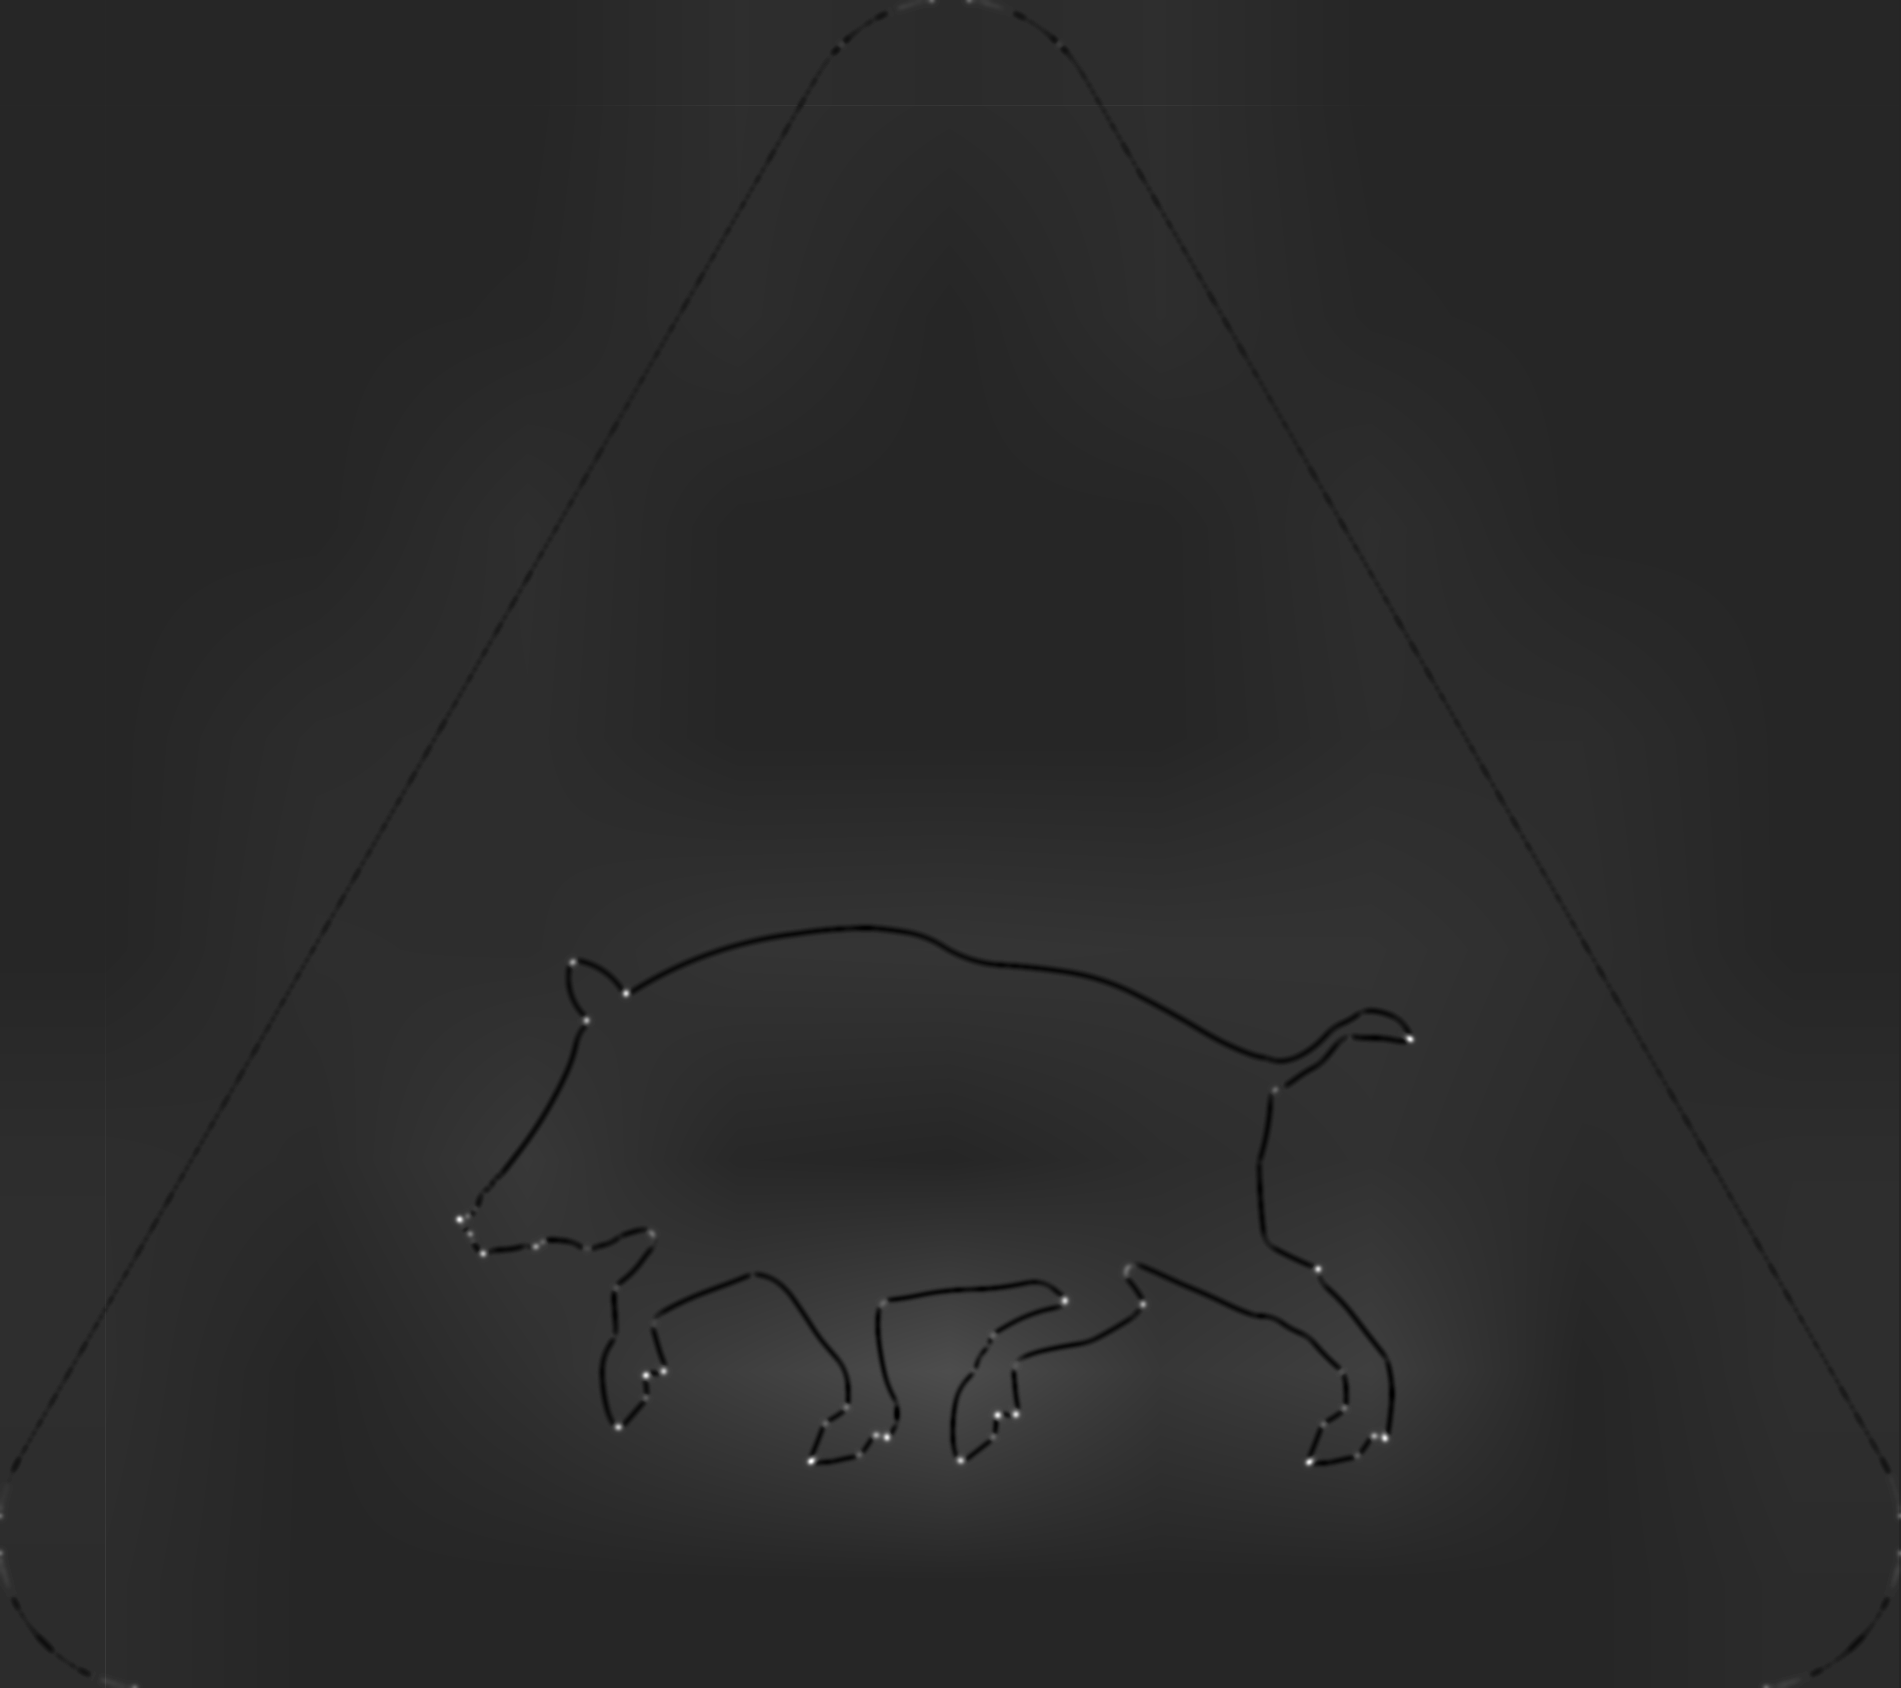
\includegraphics[width=.4\linewidth]{cornerness_swedenroad.python.png}}\hfill
\subfloat[Corner points.]{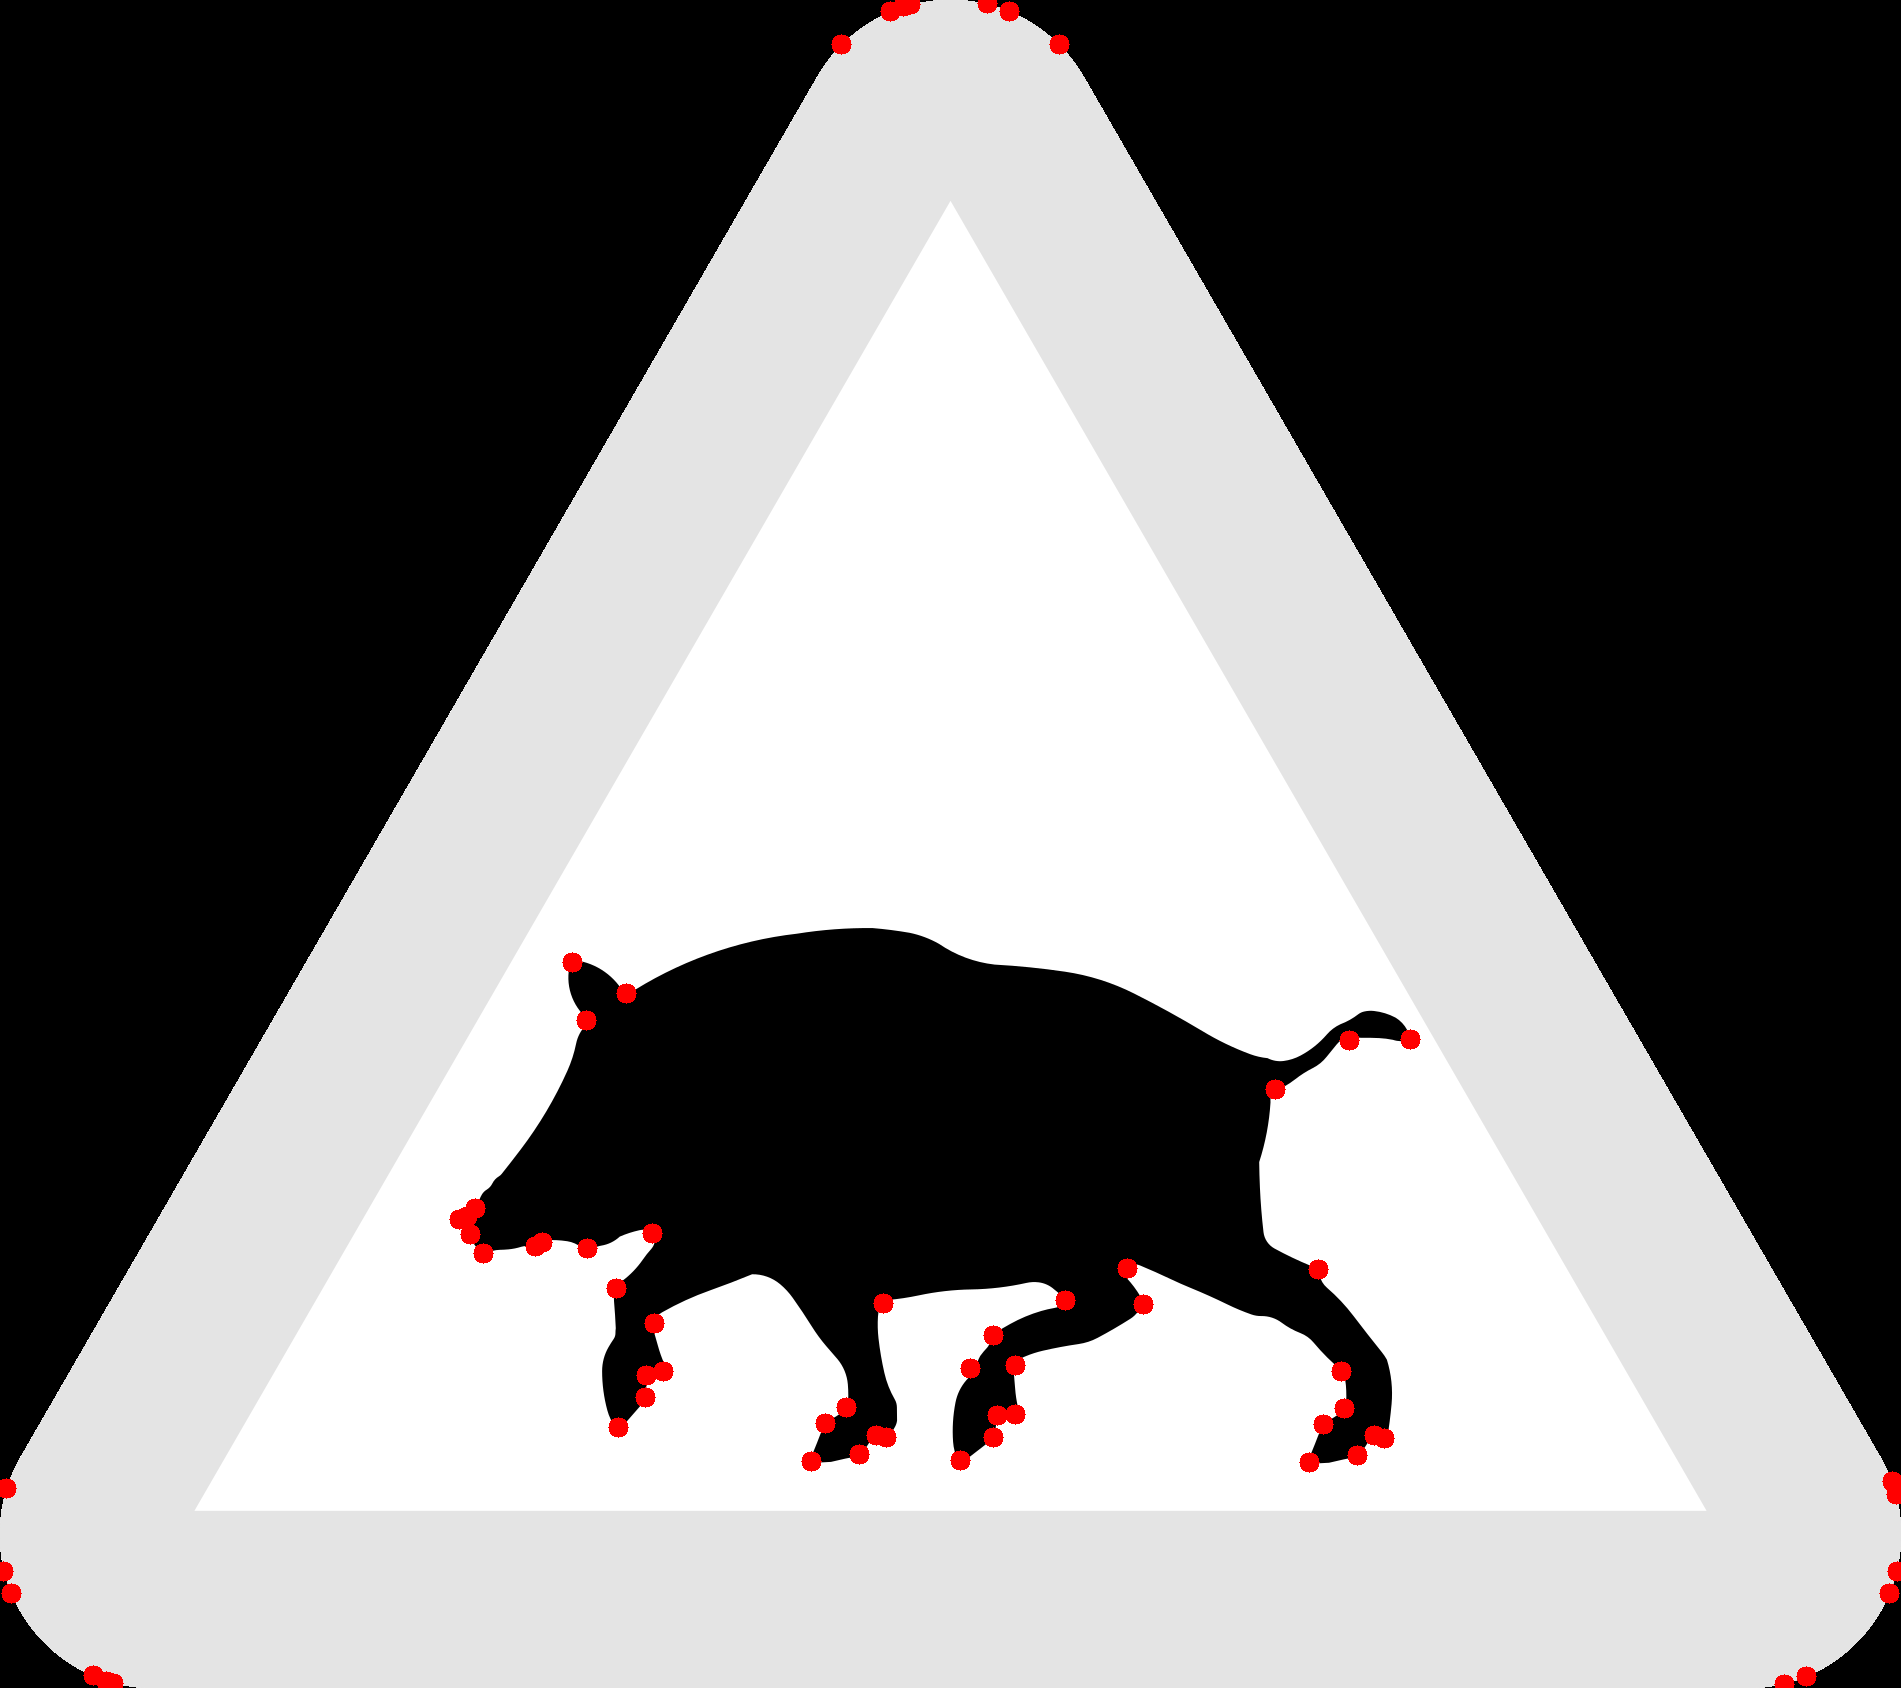
\includegraphics[width=.4\linewidth]{harris_swedenroad.python.png}}%
\label{fig:harris:python:roadsign}%
\end{figure}
